\documentclass[./../../paper.tex]{subfiles}
\graphicspath{{\subfix{./../../figures/}}}

\begin{document}

\section{Determine the Mutation-Rates}

\subsection{Experimental Setup}
\label{sec:exp2}
% We now explore optimal parameter settings. Therefore, we run the model \attention{50} times with different mutation-rates. For the chosen, we uniformly sample the mutation rates for \emph{delete}, \emph{insert} and \emph{change} between 0 and 1 for each run. The remaining procedure follows the process described in \autoref{sec:exp1}.


\subsection{Results}
% To avoid confusion, we refer to each triplet consisting of \emph{delete}, \emph{insert} and \emph{change} as one \emph{rate-configuration}. Hence, if we discuss a number of rate-configurations, we discuss a set of triplets.  

\begin{figure}[htbp]
    \centering
    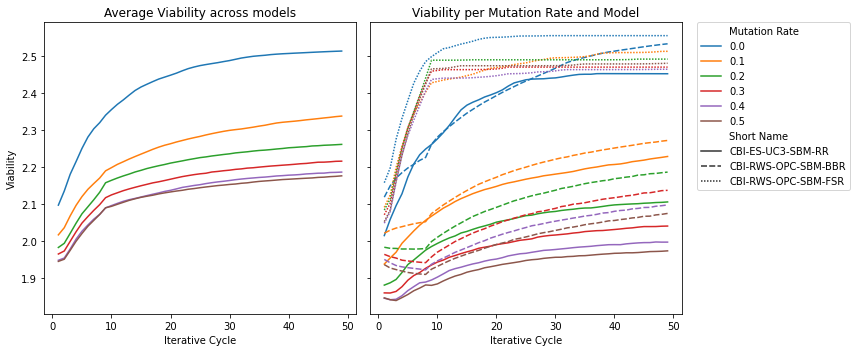
\includegraphics[width=\textwidth]{figures/generated/exp2_viability_by_mrate_model.png}
    \caption{This figure shows the viability for each model and mutation rate per iterative cycle. The first plot shows the average across models. The second figure shows the same information per model. The x-axis shows how the viability evolves for each evolutionary cycle. The color indicates the mutation rate. The line-type marks each model tested.}
    \label{fig:average-mutation-rates}
\end{figure}


\noindent As we can see in \autoref{fig:average-mutation-rates}, that a mutation rate of 0 yields better results on average. Suggesting that mutating the children might impede the model. 
For model-configurations that use the Fittest-Survivor-Recombination we observe a sharp apattern of convergence before the 10th iterative cycle.  

\input{./../../multifigures/exp2_measure_params.tex}


\subsection{Discussion}
While it is expected, that every rate-configuration eventually converges towards an optimal value, it remains surprising that most rate-configurations suddenly converge around the 10 iteration. There are a multitude of possible reasons for this phenomenon. As the viability measure incorporates structural information and event-related information, we assume that the algorithm focuses on finding a structural optimum first. Hence, the algorithm first optimizes similarity, sparcity and delta, before focusing on feasibility. This behaviour is reinforced by the viability measures' tendency to favor shorter sequences first. This phenomenon is discussed further, when we look at the event and feature structure of the results in \autoref{sec:exp4}.


However, as we have to choose a rate-configuration, we take the configuration which not only yields the highest viability but also does not converge. Therefore, we maintain the models ability to still improve beyond \attention{50} iteration cycles.
We move forward with a delete-rate of \attention{0.14}, an insert rate of \attention{0.21} and a change rate of \attention{0.23}.

\end{document}